% Why prediction is important?
\label{sec:prediction}
There is no need to change compiler instrumentation of \Predator{} to support prediction.
This section talks about why prediction is important and how to support it in runtime system.  

\subsection{Overview}
%\begin{figure*}[!htb]
\label{sec:predictoverview}

\begin{figure}[!h]
\begin{center}
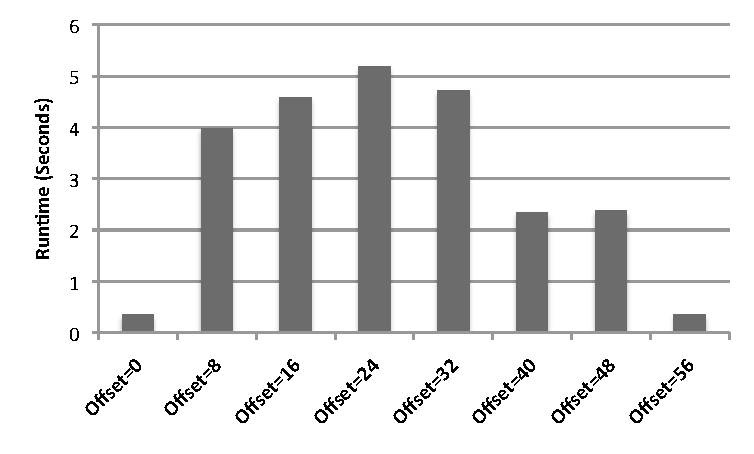
\includegraphics[width=3.3in]{fig/perfsensitive}
\end{center}
\caption{
Inside \texttt{linear\_regression} benchmark,
performance is sensitive to the offset between starting address of the false sharing object 
and the starting of cache line 
\label{fig:perfsensitive}}
\end{figure}

Occurrences of false sharing highly depend on 
alignments between objects and corresponding cache lines.
We can see an example in Figure~\ref{fig:perfsensitive}, \texttt{linear\_regression} 
benchmark evaluated in Section~\ref{sec:evaluation}. 
For this benchmark,
when the offset of starting address between the false sharing object and corresponding cache lines 
is $0$ or $56$ bytes, 
there is no false sharing problem in this benchmark. 
When the offset is $24$ bytes, we see the most severe performance effect caused 
by false sharing problem. 
The performance difference between these two can be as large as $15\times$.
%None of existing detection tools considers this manifestpossibility caused by alignments. 
Existing detection tools can only report those manifested false sharing at best. 
For this example, they may miss a very severe false sharing problem if the offset of starting 
address is actually $0$ bytes or $56$ bytes in their test environment.
\Predator{} overcomes this shortcoming by predicting potential false sharing accurately. 

\begin{figure*}
\begin{center} 
\subfigure[No false sharing]{%
   \label{fig:nofs}
   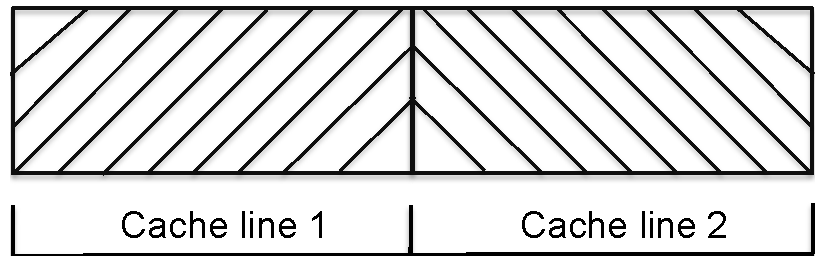
\includegraphics[width=0.24\textwidth]{fig/Potential1}
}%
\hspace{30pt}
\subfigure[False sharing with larger cache size]{%
   \label{fig:fslarger}
   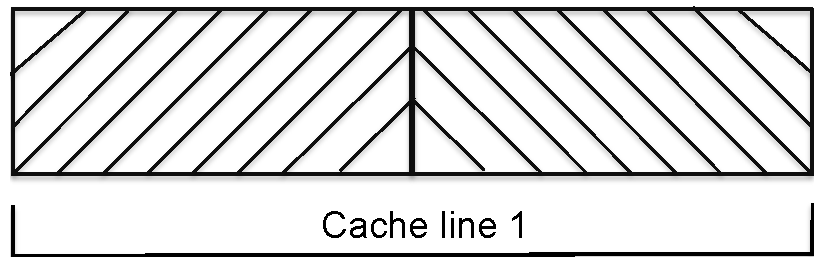
\includegraphics[width=0.24\textwidth]{fig/Potential2}
}%
\hspace{30pt}
\subfigure[False sharing with different alignment]{%
   \label{fig:fsnoalignment}
   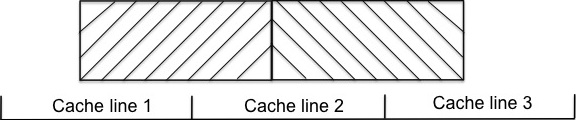
\includegraphics[width=0.36\textwidth]{fig/Potential3}
}%
\end{center}
%\includegraphics{fig/potential.pdf}
\caption{Occurrences of false sharing change under different environment}
\label{fig:potentialfalsesharing}
\end{figure*}

\Predator{} predicts {\it potential false sharing}, the type of
false sharing that does not 
manifest in current execution but may appear and greatly affect programs' performance
in a slightly different environment.

Figure~\ref{fig:potentialfalsesharing} shows a simplified example why occurrences of false sharing 
can change in different situations.
In this figure, two rectangles with different patterns
represents two portions of the same object, updated by different threads. 
In Figure~\ref{fig:nofs}), there is no false sharing when thread T1 only updates 
``cache line 1'' and T2 only updates ``cache line 2''.
However, false sharing appears in one of the following cases, even with the same
access pattern. 

\begin{itemize}
\item
Doubling cache line size (Figure~\ref{fig:fslarger}). When the size of a
cache line doubles,
T1 and T2 access the same cache line. False sharing occurs in this case.

\item
Different starting address of an object(Figure~\ref{fig:fsnoalignment}). 
When the starting address of this object is not aligned with the starting address of 
the first cache line, 
then T1 and T2 can update the second cache line simultaneously, 
causing false sharing problems. 
%When some dynamic property changes the starting address of this object so that it 
%is not aligned with the starting address of the first cache line, 
\end{itemize} 

\Predator{} predicts whether programs can have potential false sharing problems  
in any of these two cases, where they can be caused by different dynamic properties 
discussed in Section~\ref{sec:intro}.
All dynamic properties, except change of cache line size,
can lead to different starting address of an object. 
Thus, predicting false sharing in these two cases actually 
explores many possibilities caused by all dynamic properties.

\subsection{Basic Workflow of Prediction}
\label{sec:predictionmechanism} 

Similar to the detection part, 
\Predator{} only cares about those potential false sharing that can 
cause performance problems.
The implementation is based on
two important observations. First, only accesses to 
adjacent cache lines can form potential false sharing, 
i.e., introducing cache invalidations when cache line size
or an object's starting address changes.
Second, only those false sharing introducing a large amount of cache invalidations
can degrade performance.

Based on these two observations, \Predator{} develops 
the following workflow to capture potential false sharing.
Those detection optimizations listed in Section~\ref{optimization} can also be applied
to prediction part. We do not repeat these optimizations in
this whole section.

\begin{enumerate}
\item
Track the number of writes on different cache lines. 

\item
When the number of writes to a cache line $L$ reaches {\it Tracking-Threshold},
track the detailed read and write accesses for every word on both cache line $L$ 
and its adjacent cache lines. 

\item
When the number of writes to a cache line $L$ reaches a second threshold (called as
{\it Predicting-Threshold}), 
identify whether there exist false sharing problems on $L$ and its adjacent 
cache lines by analyzing word accesses information collected in Step 2. 
Section ~\ref{sec:evaluatingfs} describes the evaluation method.

\item
If a potential false sharing is found, continue to track cache line invalidations
to confirm it. Section~\ref{sec:tracking} discusses the details.
Otherwise, go back to Step 2 to track more detailed accesses.
 
\end{enumerate}

\subsection{Searching for Potential False Sharing}
\label{sec:evaluatingfs}
To describe potential false sharing problems in two different cases, 
we first introduce a virtual line concept:
{\it a virtual line is a contiguous memory range with a certain size}.
In the case of double cache line size, a virtual line 
is composed of two original 
contiguous cache lines and the first cache line has an even index number.
Thus, only cache line $2*i$ and $2*i+1$ can form a virtual line.
In the case of different starting address,
a virtual line has the same cache line size as original lines, but
flexible starting address.
Its starting address does not need to be multiple of cache line size.
For instance, a virtual line can be consisted of $[0,64)$ bytes or $[8,72)$ bytes 
for $64$ bytes of cache line.

To search for potential false sharing problems, 
\Predator{} searches for a hot access pair on $L$ and its adjacent cache lines 
by analyzing detailed word access information collected in Step 2. 
A hot access in a cache line refers to the word whose number of read or write accesses 
is larger than the average number of accesses on each word of cache line $L$.
For every hot access $X$ in cache line $L$, \Predator{} searches another
hot access $Y$ in $L$'s previous cache line or next cache line satisfying with
the following conditions: 

\begin{itemize}
\item
$X$ and $Y$ fall into the same virtual line. 

\item
One of $X$ and $Y$ is a write access.

\item 
$X$ and $Y$ are issued by different threads.

\end{itemize}

% why it finds a pair of $X$ and $Y$ == a potential false sharing 
Whenever it finds a pair of $X$ and $Y$, 
\Predator{} identifies a potential performance degrading false sharing problem
that the number of cache invalidations caused by $X$ and $Y$, at a possible virtual line, 
can be larger than the average number of accesses on each word of $L$. 
This is based on a similar observation as its prediction:
{\it if a thread writes a virtual line after other threads 
have accessed the same virtual line, this write operation most likely causes at least a cache 
invalidation}. 
However, it is impossible to know exactly how many cache invalidations occur on a virtual
line, without knowing actual access sequence of different threads.  
\Predator{} makes a conservative assumption that 
accesses from different threads are issued in an interleaving way.
This ensures we don't miss any potential false sharing as well as 
not reporting false positives.

According to above observation and assumption, 
a pair of hot accesses, $X$ and $Y$, if accesses are issued in an interleaving 
way, can generate the number of cache invalidations equaling to 
the smaller number of accesses of $X$ and $Y$.
Thus a false sharing problem is to be identified by \Predator{}.
  
After identifying possible false sharing, \Predator{} goes to Step 4 to 
verify whether this is an actual false sharing problem.

\subsection{Verifying Potential False Sharing}
\label{sec:tracking}

\Predator{} verifies potential false sharing by tracking 
cache invalidations on a problematic virtual line.
%covering a pair of hot accesses found
%in Step 3.

For potential false sharing caused by double cache line size, as described in
last section~\ref{sec:evaluatingfs}, a virtual line is always composed of 
cache line with index $2*i$ and $2*i+1$. 
\Predator{} tracks cache invalidations
on the virtual line on which false sharing has been discovered.

However, for the case with starting address change, 
two hot accesses with distance less than cache line size 
can form multiple virtual lines. 
So there is an additional step to determine which virtual line to be tracked.
Although the virtual line to be chose here is never be a real cache line of actual hardware
due to unaligned addresses,
we utilizes this virtual line to simulate the effect of changing the 
starting addresses of objects.


\begin{figure}
\begin{center} 
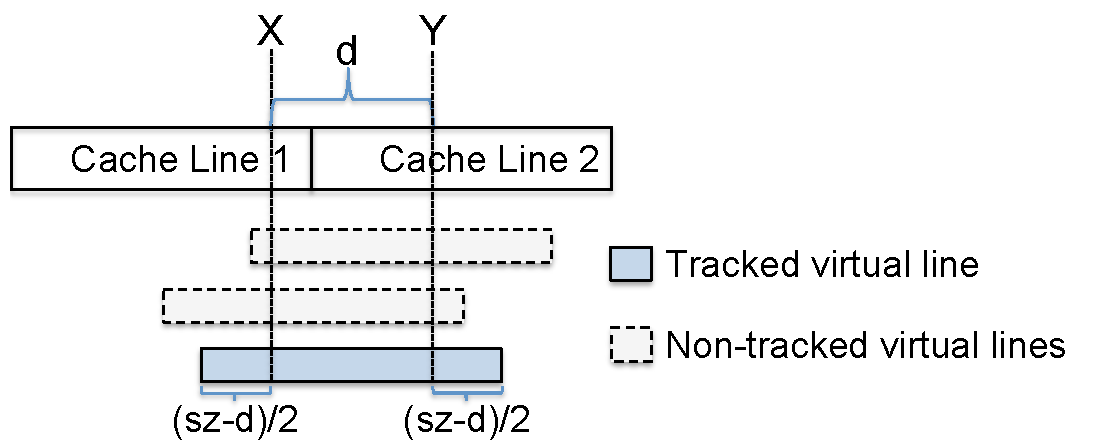
\includegraphics[width=3.3in]{fig/trackpotential}
\end{center}
\caption{Determining a virtual line with size $sz$ according to hot accesses.}
\label{fig:trackpotential}
\end{figure}

Given two words having hot accesses showed in Figure~\ref{fig:trackpotential}, 
\Predator{} leaves the same space before $X$ and after $Y$ in determining a virtual line. 
That is, the virtual line starting 
at location $X-((sz-d)/2)$ and ending at $Y+((sz-d)/2)$ is tracked. 
This choice allows to track more possible cache invalidations caused by
adjacent accesses of $X$ and $Y$. 
Since adjusting the starting address of a virtual line has the same effect of
adjusting the starting address of an object in detecting false sharing, thus
all cache lines related to the same object must be adjusted in the same time.
\Predator{} then tracks cache invalidations based on these adjusted virtual lines.

\subsection{Reporting Potential False Sharing}
Reporting potential false sharing problems shares the same mechanisms and optimizations 
of detection part.
They are discussed in Section~\ref{sec:runtime}.

